% !TEX program = xelatex
% Style học từ D:\AI_RTR\Realtime-Robotics\docs\slides\turn_7\slide.tex
% Nguyên tắc: ít chữ. Hình/bảng nói số; chữ chỉ nói NGHĨA, một câu ngắn.
\documentclass[aspectratio=169,10pt]{beamer}

\usetheme{metropolis}
\metroset{sectionpage=progressbar, numbering=fraction, block=fill, progressbar=frametitle}
\usefonttheme{professionalfonts}

\usepackage{fontspec}          % giữ XeLaTeX cho tiếng Việt
\setsansfont{Segoe UI}
\setmonofont{Consolas}
\usepackage{fvextra}
\usepackage{booktabs}
\usepackage{colortbl}          % \rowcolor
\usepackage{xcolor}
\graphicspath{{figs/}}

% ---- Màu ngữ nghĩa, mượn từ deck tham chiếu ----
\newcommand{\good}[1]{\textcolor{green!45!black}{\textbf{#1}}}   % kết quả chốt / khẳng định
\newcommand{\weak}[1]{\textcolor{red!70!black}{\textbf{#1}}}     % điểm yếu / lệch chuẩn
\definecolor{hirow}{HTML}{E4F1EC}                                % nền hàng punchline

% Câu chốt: MỘT dòng ngắn, xanh, canh đáy khung
\newcommand{\take}[1]{\vfill{\footnotesize\textcolor{green!45!black}{#1}}}

\newcommand{\promptbox}[2]{\VerbatimInput[breaklines=true,breakanywhere=true,%
  breaksymbolleft={},breakautoindent=true,%
  fontsize=#1,baselinestretch=0.92,frame=single,framesep=4pt,%
  rulecolor=\color{black!35},formatcom=\color{black!85}]{#2}}

\title{Tác nhân LLM trong trò chơi rủi ro tập thể --- Turn 1}
\subtitle{Tái lập Milinski et al.\ (2008): prompt · kết quả · cơ chế}
\date{\today}
\author{Báo cáo nghiên cứu}

\begin{document}
\maketitle

% ======================================================================
\section{Bối cảnh}

\begin{frame}{Trò chơi rủi ro tập thể (Milinski 2008)}
  \begin{columns}[T]
    \begin{column}{0.57\textwidth}
      \textbf{Luật chơi}
      \begin{itemize}\setlength\itemsep{3pt}
        \item 6 người chơi, mỗi người vốn 40
        \item 10 vòng; mỗi vòng đóng \{0, 2, 4\} vào quỹ chung
        \item \alert{Mục tiêu nhóm}: tổng $\geq 120$
        \item Không đạt $\Rightarrow$ xác suất $p$ cả nhóm \alert{mất sạch}; đạt thì giữ phần chưa đóng
        \item Rủi ro $p \in \{0.9,\ 0.5,\ 0.1\}$
      \end{itemize}
    \end{column}
    \begin{column}{0.40\textwidth}
      \textbf{Người thật làm gì?}
      \smallskip
      \begin{center}
      \setlength{\tabcolsep}{9pt}\renewcommand{\arraystretch}{1.2}
      \begin{tabular}{cc}
        \toprule
        Rủi ro & Tỉ lệ đạt \\
        \midrule
        0.9 & 50\% \\
        0.5 & 10\% \\
        0.1 & \phantom{0}0\% \\
        \bottomrule
      \end{tabular}
      \end{center}
      \take{Người \emph{hợp tác nhiều hơn khi rủi ro cao} --- nhạy với rủi ro.}
    \end{column}
  \end{columns}
\end{frame}

\begin{frame}{Bốn điều kiện, ba mô hình}
  \centering
  \setlength{\tabcolsep}{10pt}\renewcommand{\arraystretch}{1.3}
  \begin{tabular}{lll}
    \toprule
    Điều kiện & Thao tác & So với baseline \\
    \midrule
    \textbf{1. Baseline} & (đối chứng)   & xem trọn lịch sử, trung tính \\
    \textbf{2. Memory}   & trí nhớ       & chỉ vòng gần nhất + sổ tay (giống paper) \\
    \textbf{3. Framing}  & khung tâm lý  & thêm khung ``chỉ quan tâm tiền của bạn'' \\
    \textbf{4. Persona}  & tính cách     & thêm 0$\to$6 tác nhân ``ích kỷ'' \\
    \bottomrule
  \end{tabular}
  \vfill
  \begin{block}{Ba mô hình mã nguồn mở}
    \centering Qwen2.5-7B \quad•\quad Llama-3.1-8B \quad•\quad Gemma-2-9B \\
    {\footnotesize Mỗi điều kiện: 3 mức rủi ro $\times$ \{EN, VN\} $\times$ 10 lần lặp; quyết định đồng thời, ẩn danh.}
  \end{block}
\end{frame}

% ======================================================================
\section{1 · Baseline}

\begin{frame}[fragile]{Baseline --- prompt ví dụ (vòng 3, đã có lịch sử)}
  \promptbox{\fontsize{7}{8}\selectfont}{assets/prompt_baseline_r3.txt}
\end{frame}

\begin{frame}{Baseline --- phớt lờ rủi ro (so với người)}
  \centering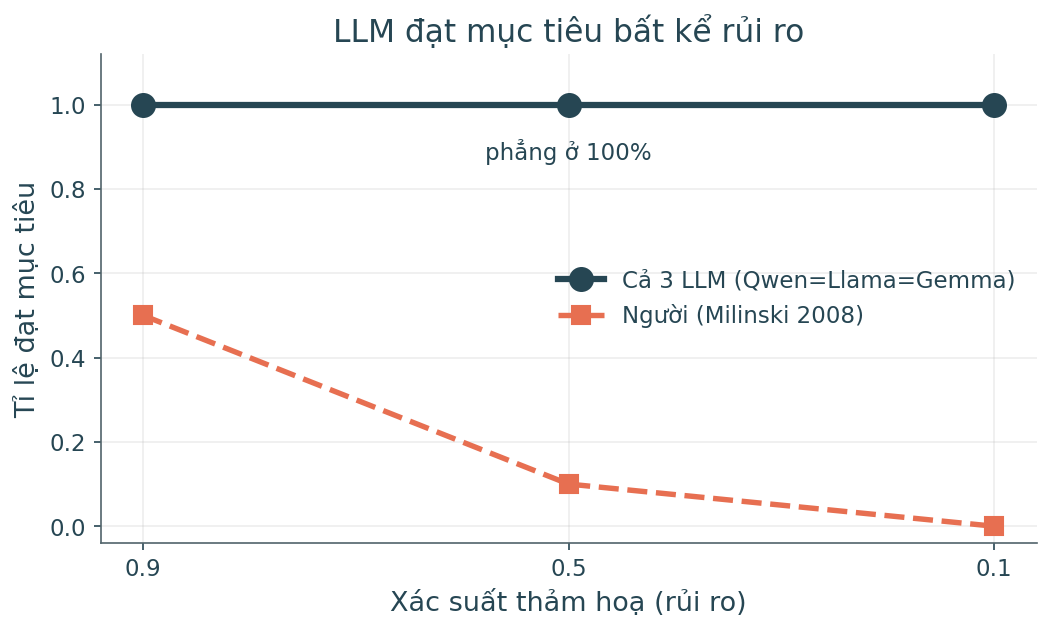
\includegraphics[height=0.70\textheight]{A_reach_vs_risk.png}
  \take{Cả 3 model đạt \good{$\sim$100\%} ở mọi mức rủi ro; người giảm 50$\to$10$\to$0\%.}
\end{frame}

\begin{frame}{Baseline --- đóng góp cũng phẳng, chỉ khác độ hào phóng}
  \centering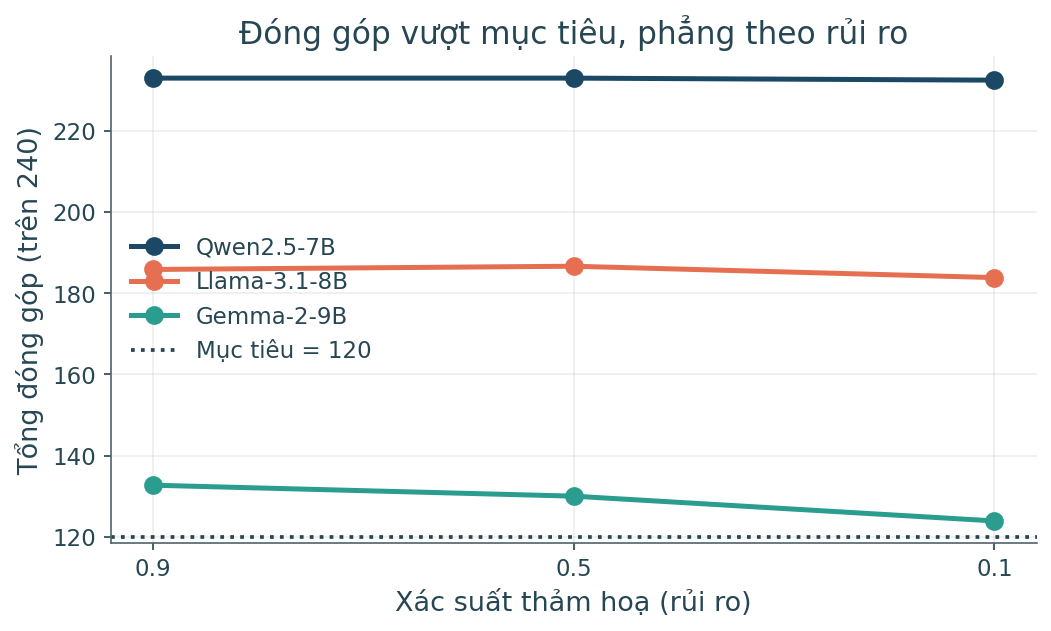
\includegraphics[height=0.66\textheight]{B_contrib_vs_risk.png}
  \take{Đóng góp không phản ứng rủi ro; hào phóng Qwen \weak{233} $>$ Llama 185 $>$ Gemma \good{129} (sát mục tiêu nhất).}
\end{frame}

\begin{frame}{Baseline --- ``vân tay'' lựa chọn của mỗi mô hình}
  \centering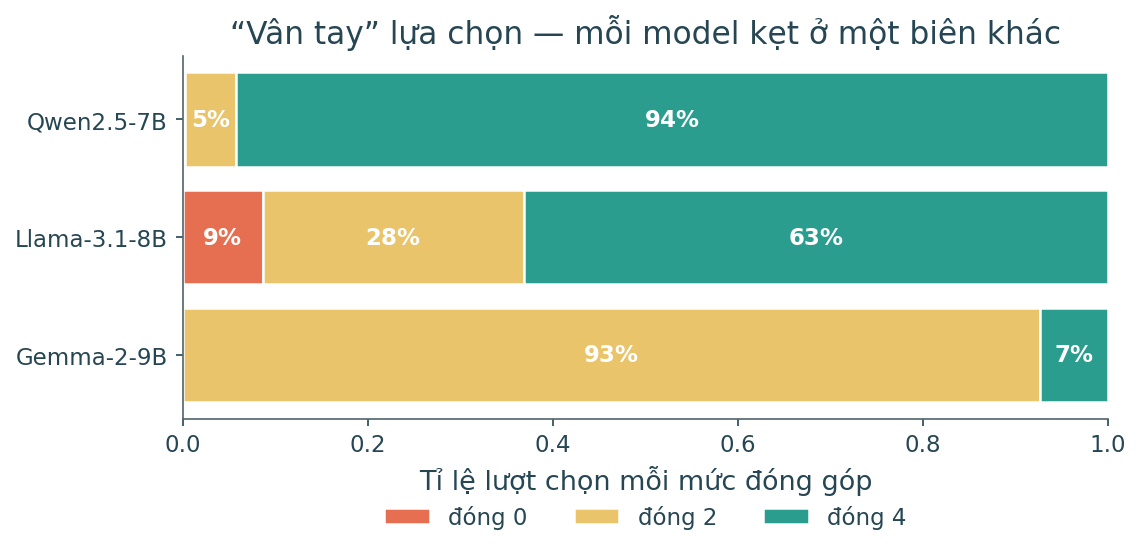
\includegraphics[height=0.64\textheight]{H_choice_dist.png}
  \take{Qwen luôn chọn 4 (\weak{94\%}, kịch trần), Gemma khoá ở 2 (93\%, kịch sàn); chỉ Llama trộn cả ba $\Rightarrow$ nhạy nhất.}
\end{frame}

\begin{frame}{Baseline --- ``vân tay'' tách theo 3 mức rủi ro}
  \centering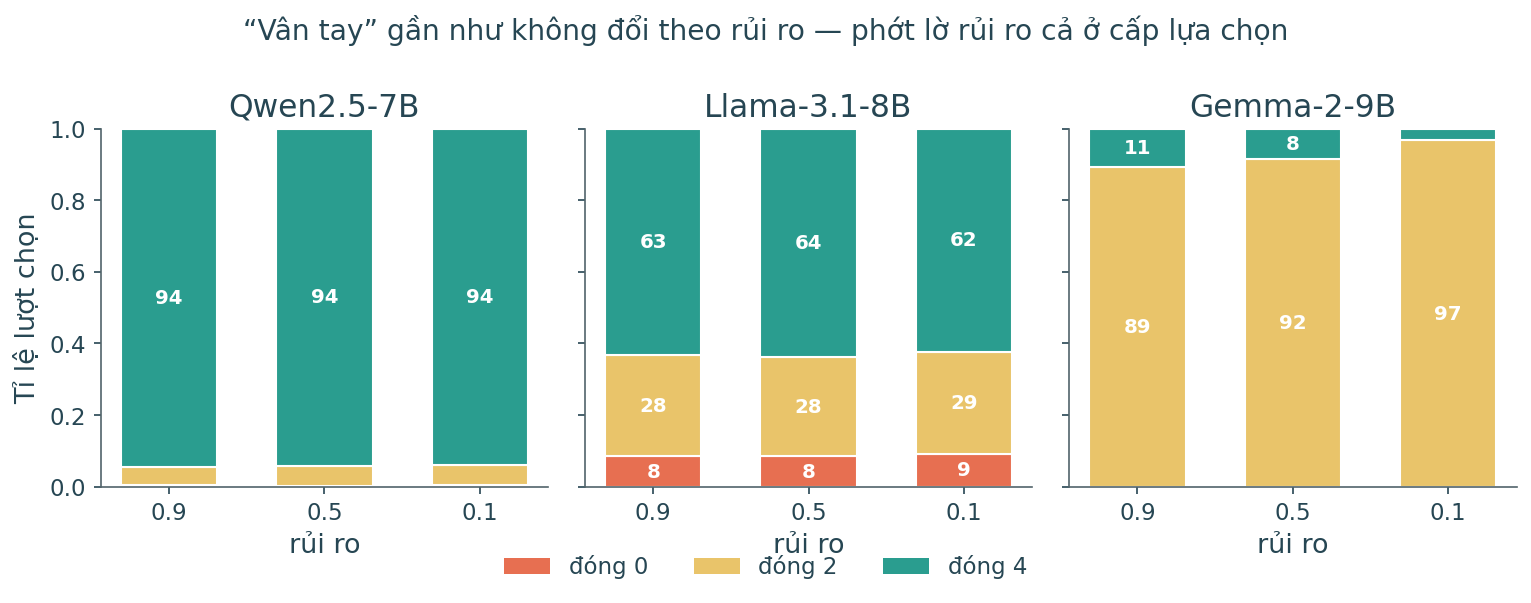
\includegraphics[height=0.62\textheight]{H2_choice_dist_risk.png}
  \take{Lựa chọn gần như đứng yên qua rủi ro (Qwen 94/94/94) --- phớt lờ rủi ro \emph{cả ở cấp lựa chọn}.}
\end{frame}

\begin{frame}{Baseline --- ngôn ngữ: tiếng Anh vs tiếng Việt}
  \centering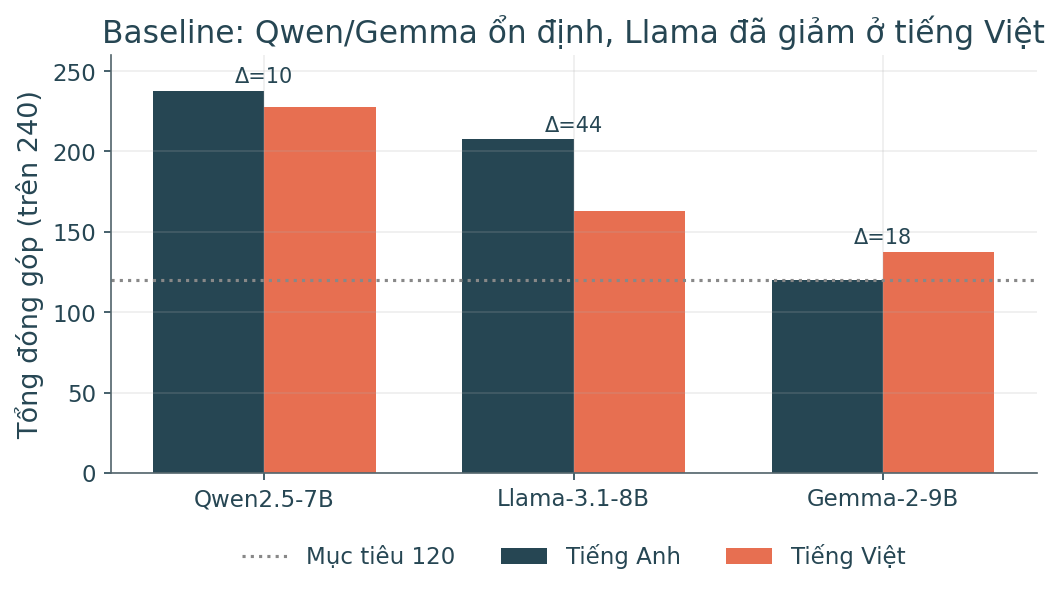
\includegraphics[height=0.66\textheight]{I_lang_baseline.png}
  \take{Reach thì EN $=$ VN (đều 100\%); nhưng đóng góp đã hé trục ngôn ngữ --- Llama giảm \weak{$\sim$44} ở tiếng Việt.}
\end{frame}

\begin{frame}{Baseline --- hợp tác TĂNG dần (ngược người)}
  \centering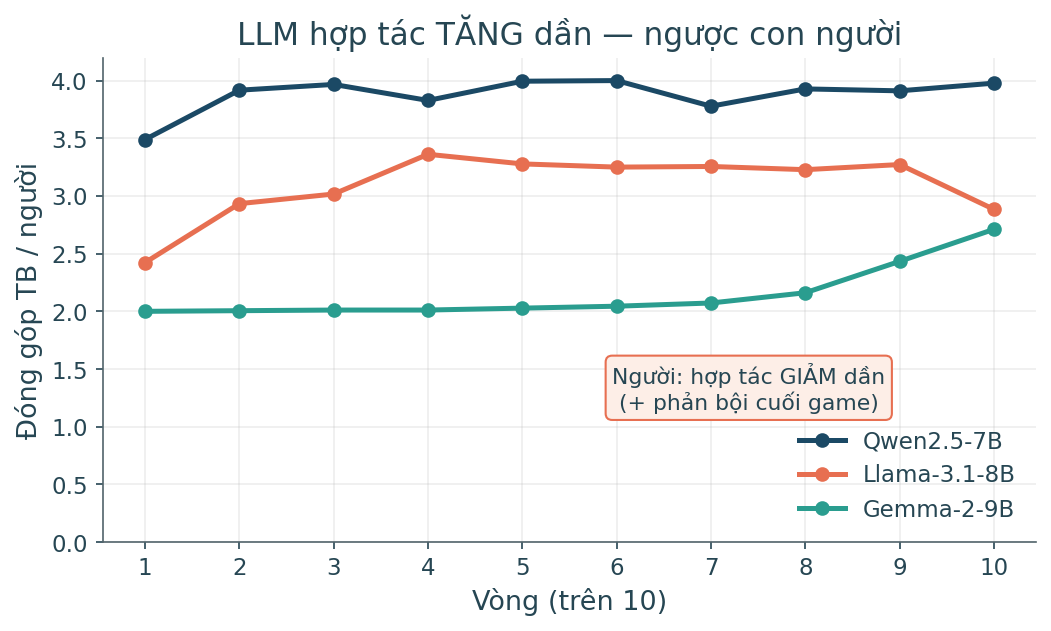
\includegraphics[height=0.66\textheight]{C_round_dynamics.png}
  \take{Người: hợp tác giảm + phản bội cuối game. LLM: \alert{tăng dần} rồi bão hoà, không phản bội.}
\end{frame}

% ======================================================================
\section{2 · Memory}

\begin{frame}{Memory --- vì sao? (theo paper gốc)}
  \begin{itemize}\setlength\itemsep{3pt}
    \item Bản gốc KHÔNG cho xem trọn lịch sử --- người chơi \textbf{tự ghi bằng giấy--bút}.
    \item Baseline (full history) là bản tiện-lợi-hoá; \alert{scratchpad mới trung thành với paper}.
  \end{itemize}
  \vfill
  \begin{exampleblock}{Trích Milinski et al.\ (2008), PNAS --- \emph{Materials and Methods}}
    \small\itshape
    ``\dots the cumulative sum of contributions was not displayed on the computer screen. Instead, the students were given pen and paper, and they were encouraged to take notes during the game.''
  \end{exampleblock}
\end{frame}

\begin{frame}[fragile]{Memory --- prompt (phần khác baseline)}
  \promptbox{\scriptsize}{assets/delta_memory.txt}
\end{frame}

\begin{frame}{Memory --- chỉ Gemma bị ảnh hưởng}
  \centering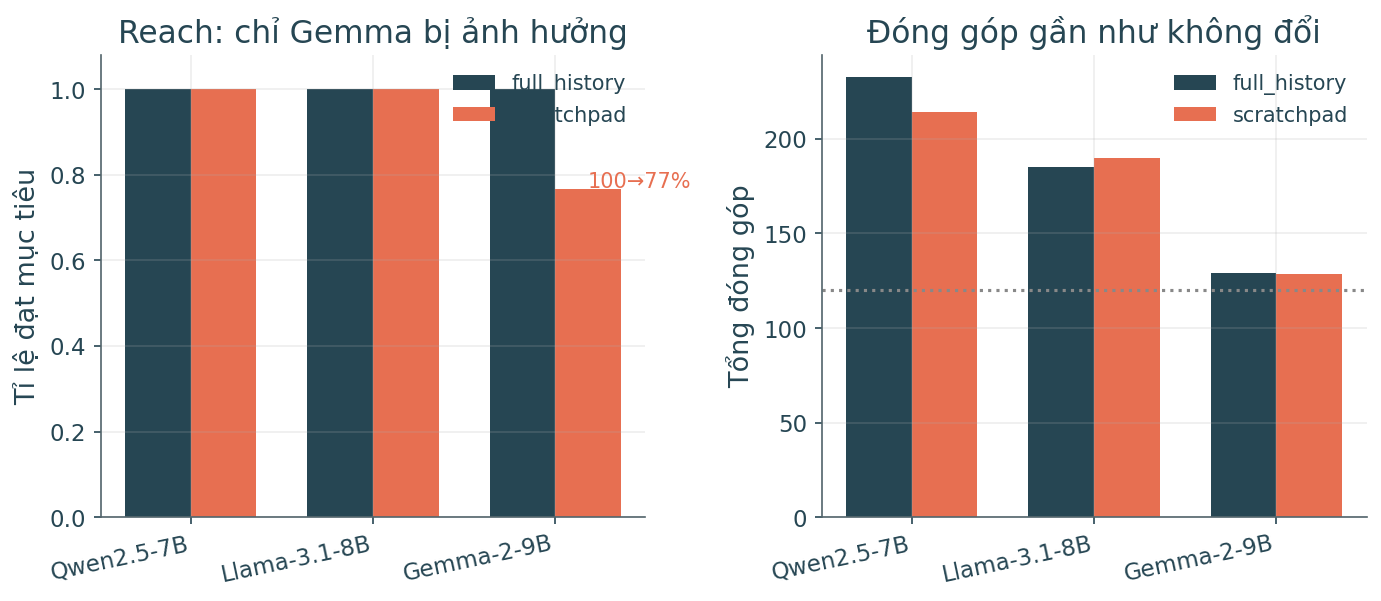
\includegraphics[height=0.66\textheight]{M_memory.png}
  \take{Trí nhớ giới hạn chỉ hại model ``sát mục tiêu'' nhất (Gemma \weak{100$\to$77\%}); Qwen/Llama dư slack nên không sao.}
\end{frame}

\begin{frame}{Memory --- động lực vòng: full-history vs scratchpad}
  \centering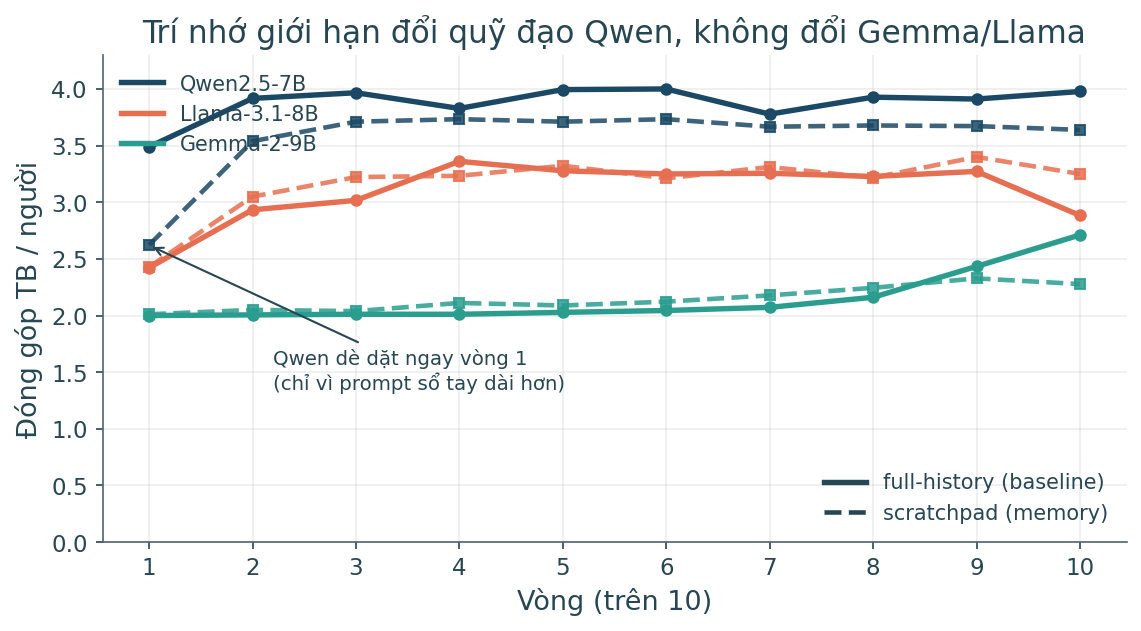
\includegraphics[height=0.66\textheight]{M2_memory_dynamics.png}
  \take{Riêng Qwen dè dặt hơn dưới scratchpad (3.49$\to$2.62) vì hướng dẫn sổ tay dài thêm; Gemma/Llama giữ nguyên quỹ đạo.}
\end{frame}

% ======================================================================
\section{3 · Framing}

\begin{frame}[fragile]{Framing --- khác baseline ở đâu?}
  \begin{block}{Thao tác --- thiết kế 2$\times$2 (framing $\times$ memory)}
    {\footnotesize Chèn \textbf{khung tâm lý ích kỷ} lên đầu prompt; luật chơi giữ NGUYÊN. Chạy trên \textbf{cả hai} chế độ trí nhớ (full-history \emph{và} scratchpad).}
  \end{block}
  \promptbox{\scriptsize}{assets/delta_framing.txt}
\end{frame}

\begin{frame}{Framing --- \emph{giảm bao nhiêu} đóng góp (mạnh hơn ở tiếng Việt)}
  \centering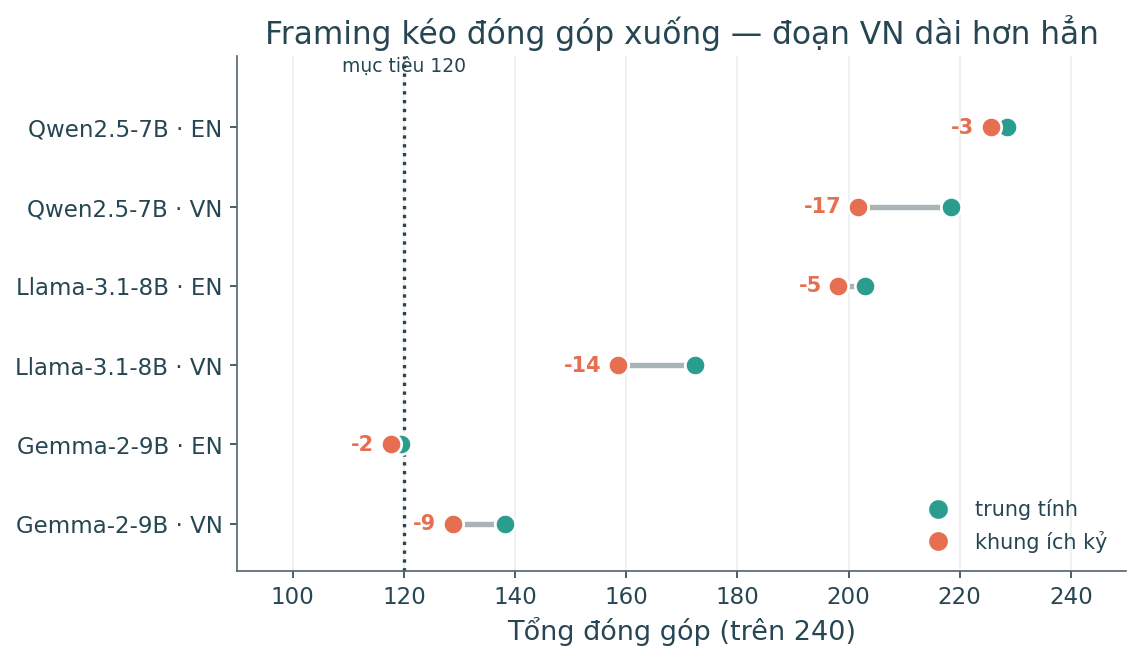
\includegraphics[height=0.66\textheight]{FR_framing.png}
  \take{Khung ích kỷ kéo đóng góp xuống cả 3 model; mức giảm ở tiếng Việt lớn hơn tiếng Anh \good{2.9--5.8$\times$}.}
\end{frame}

\begin{frame}{Framing --- \emph{ai hỏng} mục tiêu (chỉ Gemma rớt)}
  \centering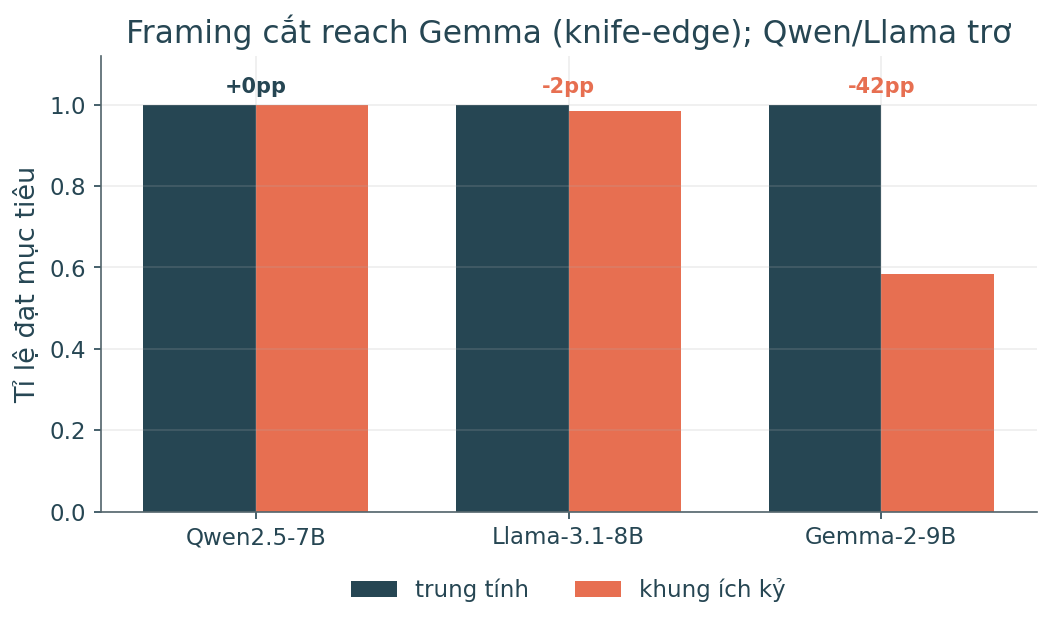
\includegraphics[height=0.66\textheight]{FR3_framing_reach.png}
  \take{Gemma rớt reach \weak{100$\to$58\%} vì chơi ngay trên vạch 120; Qwen/Llama gần như trơ. ``Dễ tổn thương'' đo bằng khoảng cách tới ngưỡng.}
\end{frame}

% ======================================================================
\section{4 · Persona}

\begin{frame}[fragile]{Persona --- khác baseline ở đâu?}
  \begin{block}{Thao tác}
    {\footnotesize Gán cho mỗi tác nhân một \textbf{dòng tính cách}. Nhóm trộn 0$\to$6 tác nhân ích kỷ (gradient), vị trí xáo trộn. Phần còn lại như baseline.}
  \end{block}
  \promptbox{\scriptsize}{assets/delta_persona.txt}
\end{frame}

\begin{frame}{Persona --- thao tác hiệu quả nhất}
  \centering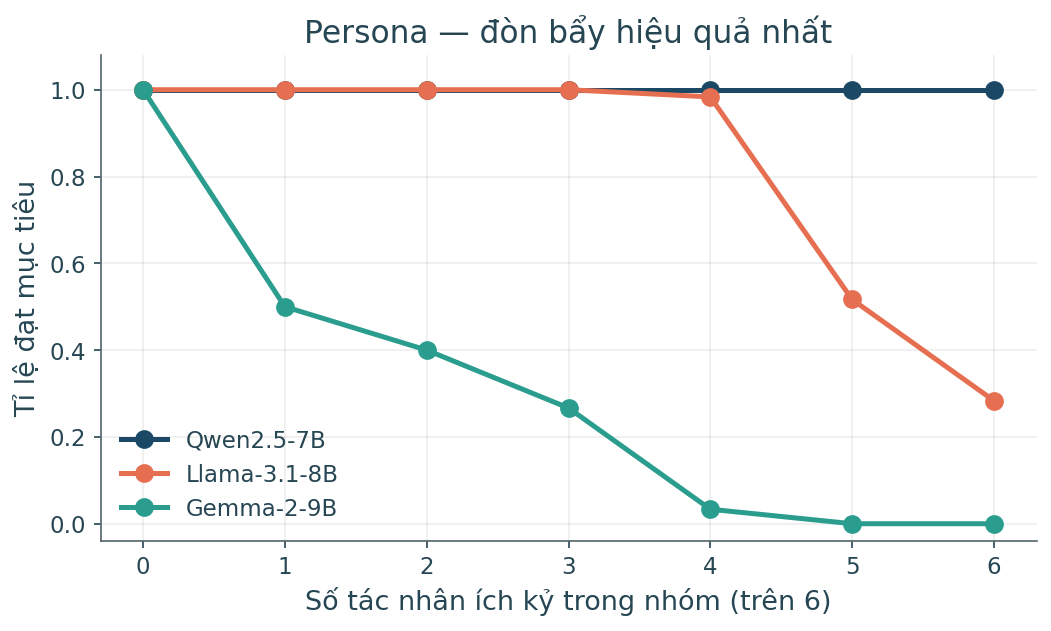
\includegraphics[height=0.66\textheight]{D_persona_reach.png}
  \take{Gemma sụp ngay ở 1 tác nhân ích kỷ; Llama ``vực thẳm'' muộn; Qwen đạt \good{100\%} \alert{ngay cả khi cả 6 đều ích kỷ}.}
\end{frame}

\begin{frame}{Persona --- reach chỉ là ``xác suất dải cắt 120''}
  \centering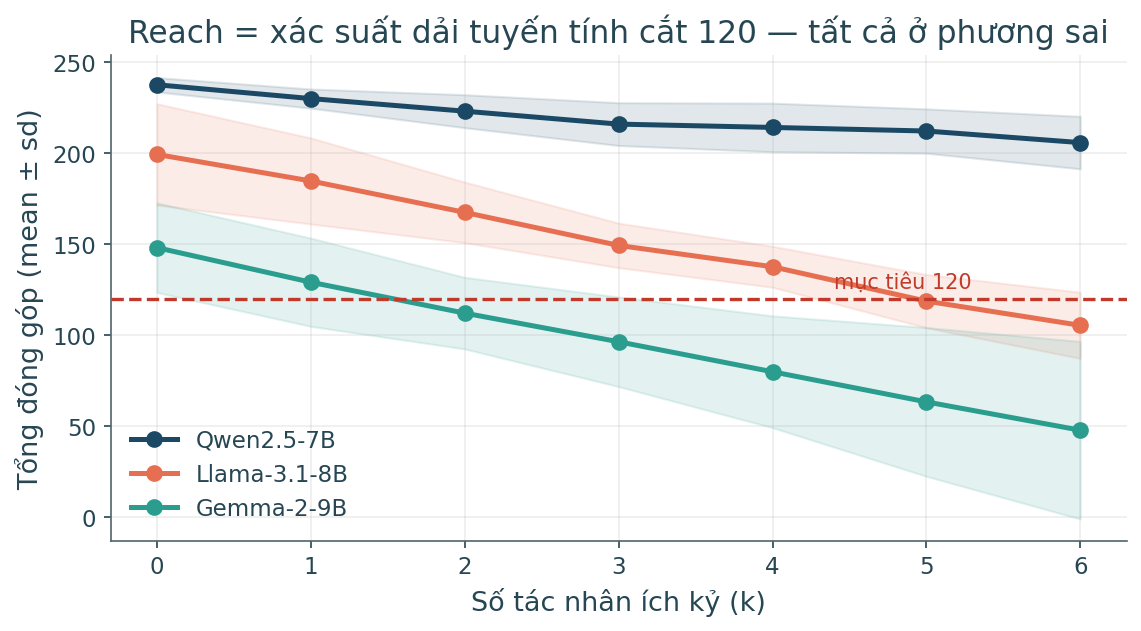
\includegraphics[height=0.66\textheight]{D2_persona_dispersion.png}
  \take{Reach kịch tính chỉ là nơi dải (mean$\pm$sd) cắt 120. Gemma ở $k{=}1$ trung bình 129 nhưng sd$\sim$24 cưỡi vạch $\Rightarrow$ \weak{$\sim$50\%} đạt.}
\end{frame}

\begin{frame}{Persona --- một động cơ tuyến tính, ba chế độ}
  \centering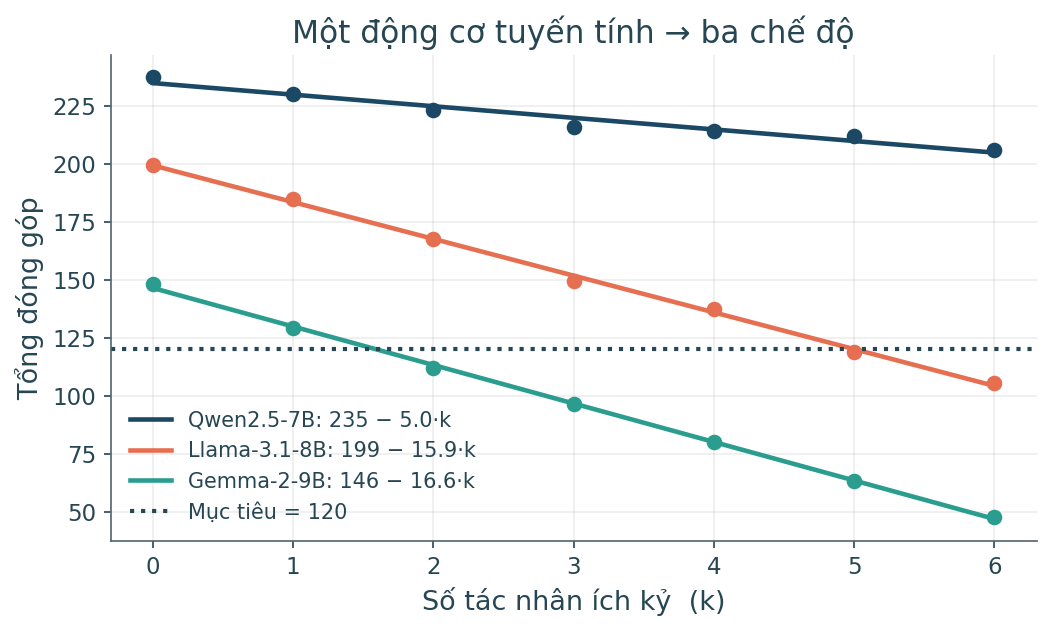
\includegraphics[height=0.66\textheight]{E_persona_linear.png}
  \take{Đóng góp giảm tuyến tính theo số tác nhân ích kỷ; đường ``đạt mục tiêu'' chỉ là nơi đường thẳng cắt 120.}
\end{frame}

\begin{frame}{Persona --- ăn ở cấp cá nhân, nhưng Qwen ít nghe}
  \centering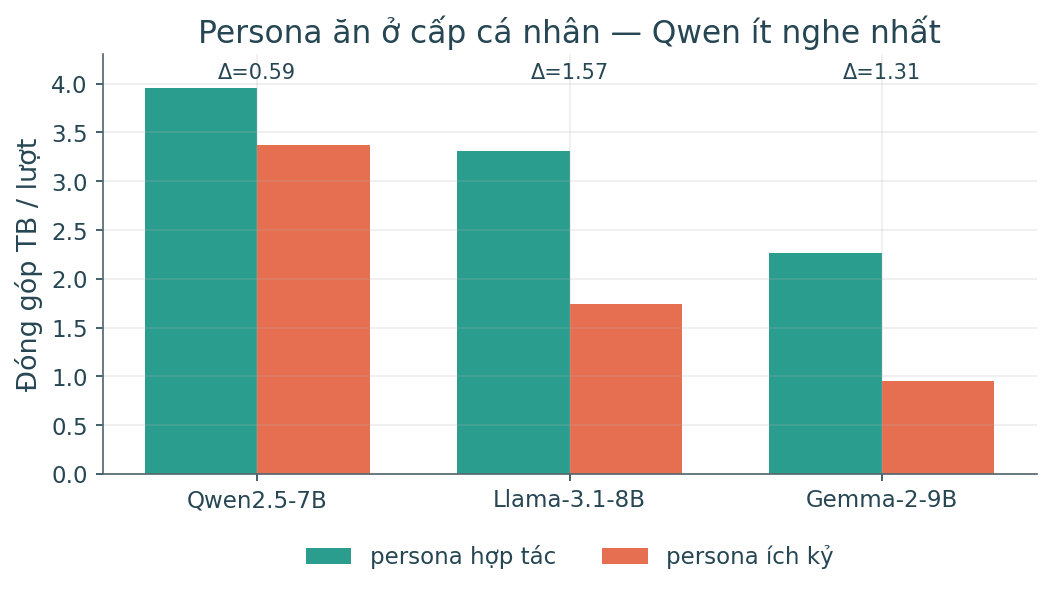
\includegraphics[height=0.64\textheight]{G_disposition.png}
  \take{Tác nhân ``ích kỷ'' của Qwen vẫn đóng \weak{3.4/4} ($\Delta$=0.59); Llama nghe lời rõ nhất.}
\end{frame}

\begin{frame}{Persona --- sụp đổ của Gemma là do tiếng Anh}
  \centering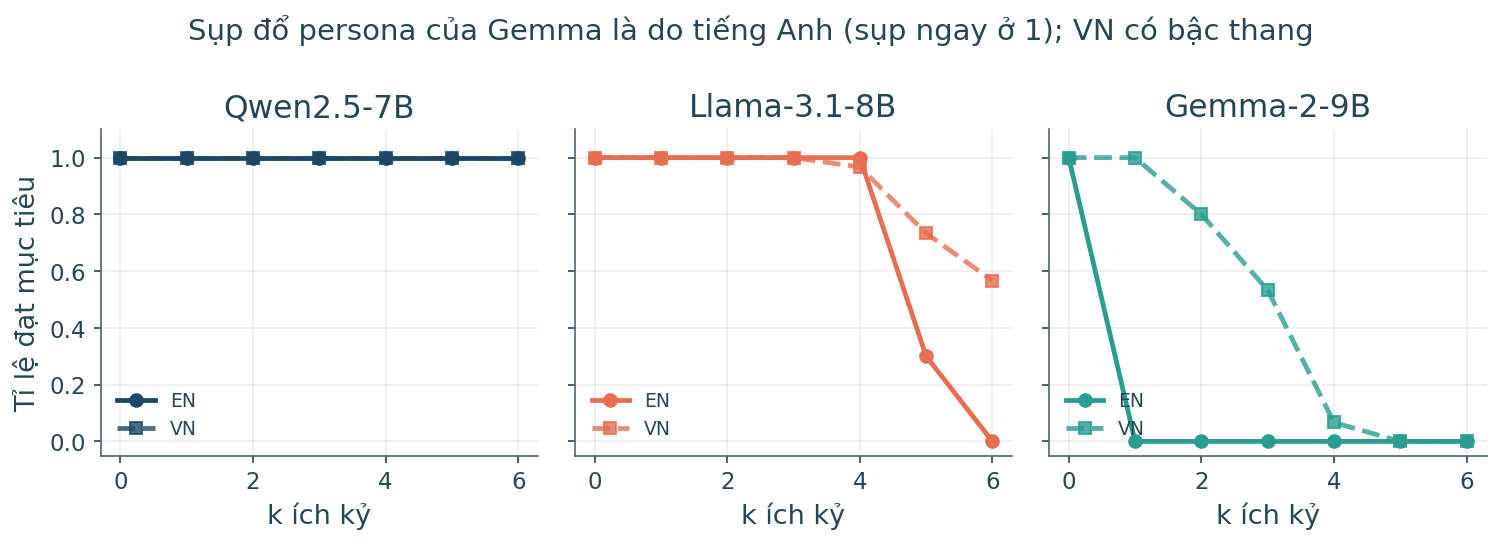
\includegraphics[height=0.62\textheight]{J_persona_lang.png}
  \take{Gemma-EN: chỉ 1 ích kỷ là reach về \weak{0\%}; Gemma-VN xuống bậc thang (100/80/53\%). Qwen trơ ở cả hai ngôn ngữ.}
\end{frame}

\begin{frame}{Persona --- kiểm chứng tính vững (vị trí ghế)}
  \centering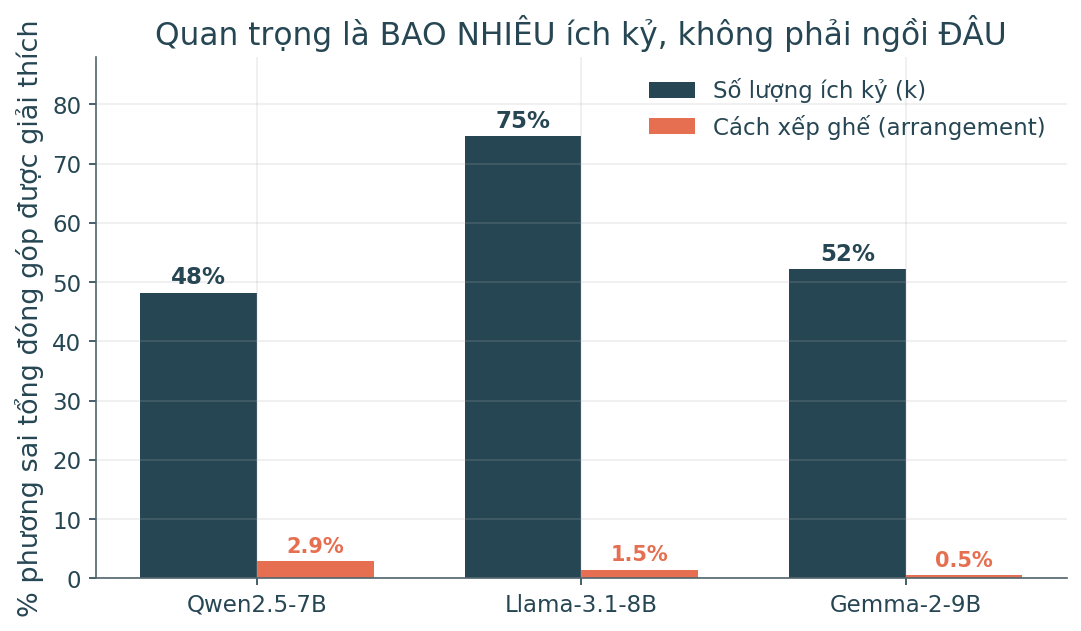
\includegraphics[height=0.64\textheight]{Q_persona_variance.png}
  \take{SỐ LƯỢNG ích kỷ giải thích \good{48--75\%} phương sai; CÁCH XẾP GHẾ chỉ 0.5--2.9\% $\Rightarrow$ dose-response không phụ thuộc vị trí.}
\end{frame}

% ======================================================================
\section{Tổng hợp}

\begin{frame}{Hiệu quả kinh tế --- ai ``khôn'' nhất?}
  \centering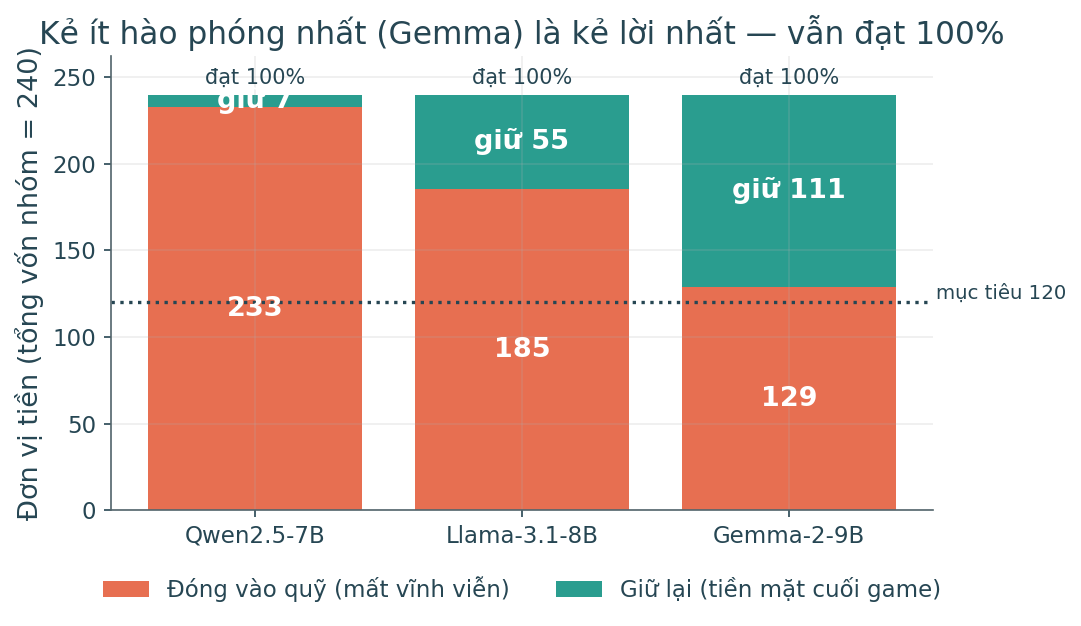
\includegraphics[height=0.64\textheight]{P_efficiency.png}
  \take{Cả ba đạt 100\%, nhưng Gemma giữ lại \good{111/240} tiền mặt, Llama 55, Qwen \weak{7} $\Rightarrow$ model ít hào phóng nhất lại tối ưu kinh tế nhất.}
\end{frame}

\begin{frame}{So với người: bảng tổng}
  \centering
  \setlength{\tabcolsep}{11pt}\renewcommand{\arraystretch}{1.35}
  \begin{tabular}{lll}
    \toprule
    Khía cạnh & Người (Milinski 2008) & LLM (cả 3) \\
    \midrule
    \rowcolor{hirow} Nhạy rủi ro        & Có (50/10/0\%) & \weak{Không} (100\% phẳng) \\
    Hợp tác qua vòng   & Giảm dần       & \alert{Tăng dần} \\
    Phản bội cuối game & Có             & \alert{Không} \\
    Mức đóng góp       & Vừa đủ         & \alert{Vượt mục tiêu} \\
    Phản ứng persona   & ---            & Có (mạnh nhất) \\
    \bottomrule
  \end{tabular}
  \take{LLM \emph{hợp tác hơn nhưng kém ``duy lý chiến lược''} so với người.}
\end{frame}

\begin{frame}{Cơ chế sâu (đã kiểm chứng đối kháng)}
  \begin{itemize}\setlength\itemsep{4pt}
    \item \textbf{``Conditional cooperation'' phần lớn là ảo}: sau kiểm soát, Qwen/Llama hợp tác \emph{vô điều kiện}, không theo dõi đối tác.
    \item \textbf{Cú ``cứu'' cuối game} của Gemma-VN là \emph{ramp theo deadline}, không phải bù trừ theo nhu cầu.
    \item \textbf{Ghi sổ sai có hệ thống}: Qwen/Llama ghi tổng chỉ \weak{$\sim$1/3} thực tế --- nhưng vẫn đạt $\Rightarrow$ hợp tác là \emph{prior}, không phải tính toán.
    \item \textbf{Trục ngôn ngữ}: bù trừ chỉ ở VN; framing nặng hơn ở VN; persona-collapse nặng hơn ở EN.
  \end{itemize}
\end{frame}

\begin{frame}{Điểm thảo luận với thầy}
  \textbf{Về prompt}
  \begin{itemize}\setlength\itemsep{2pt}
    \item Khung framing lẫn confound (\emph{có} câu mục tiêu vs \emph{không}); có cần khối neutral cân bằng?
    \item Baseline (full history) khác paper --- có nên lấy \emph{scratchpad} làm điều kiện chính?
  \end{itemize}
  \smallskip
  \textbf{Về phương pháp}
  \begin{itemize}\setlength\itemsep{2pt}
    \item \texttt{target\_reached} bão hoà 100\% $\Rightarrow$ dùng \emph{mức đóng góp} làm biến phụ thuộc chính.
    \item Lỗi nhỏ: hoán vị ghế phủ chưa đều + ``primacy'' theo nhãn \texttt{Player\_1} (ảnh hưởng <3\%).
  \end{itemize}
\end{frame}

\begin{frame}[standout]
  Tác nhân LLM: kẻ \textbf{hợp tác vô điều kiện}, \textbf{phớt lờ rủi ro}, làm \textbf{ngược đường cong người} --- và \textbf{ngôn ngữ} là trục điều tiết chính.
\end{frame}

\end{document}
